\section{Evaluation}
\label{sec:exp}
\begin{figure}[t]
\centering
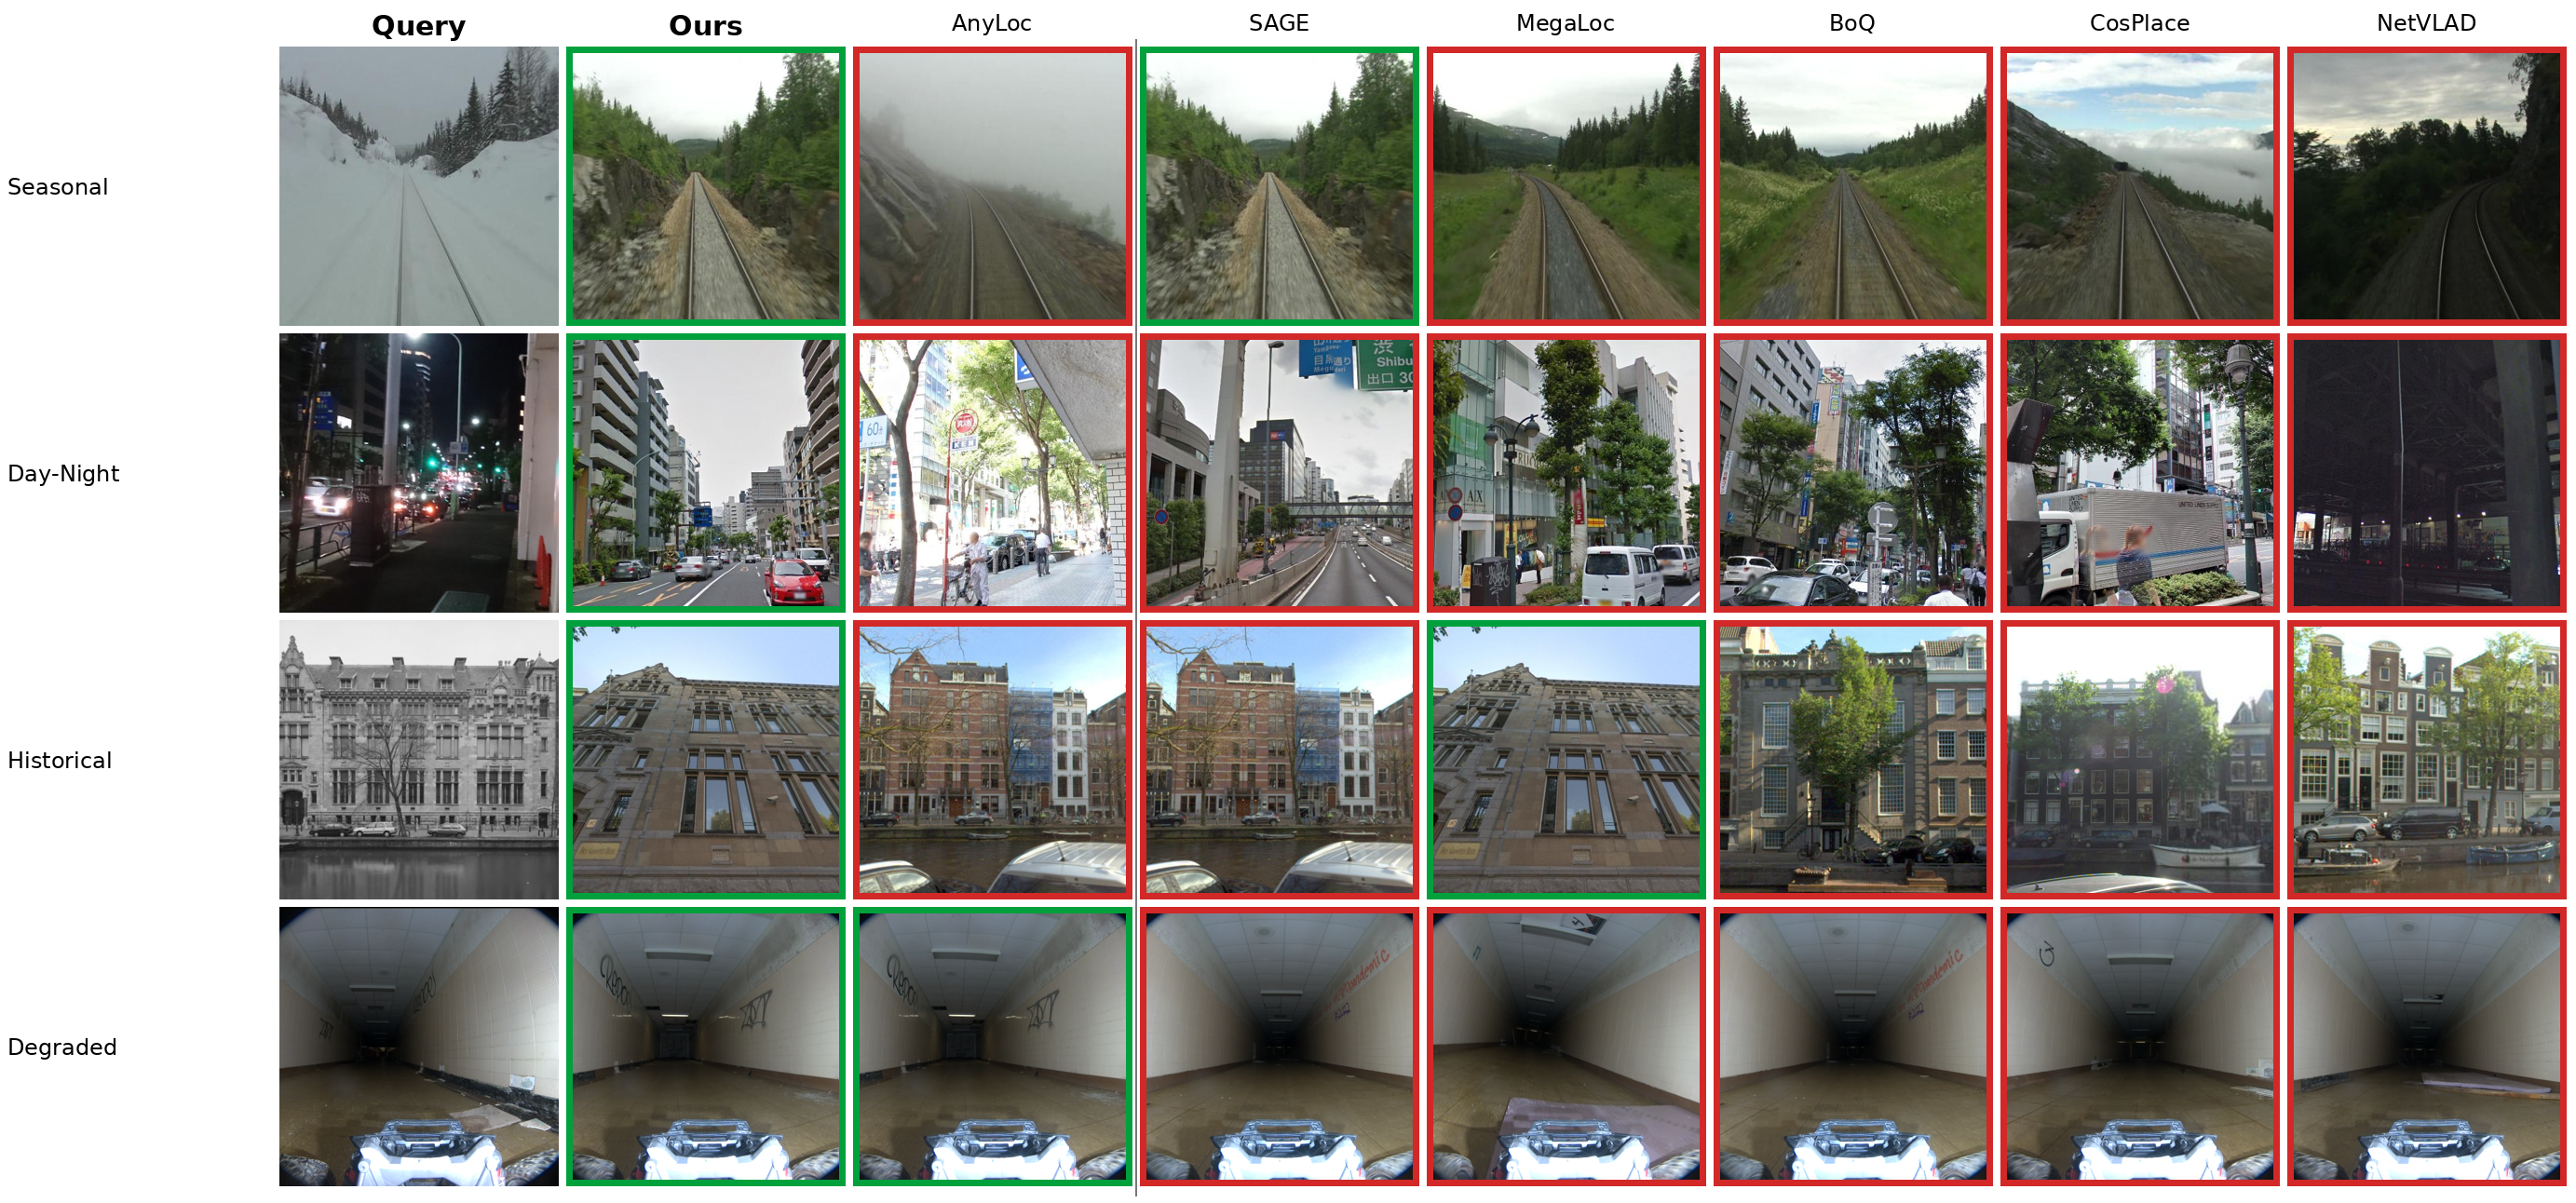
\includegraphics[width=0.82\textwidth]{figures/fig_qualitative.png}
\caption{\textbf{Rank-1 retrievals across benchmark families.} Each method at its own single stage; a green border marks a correct rank-1, red an incorrect one. Training-free methods above the line, the three strongest trained baselines below. Queries are drawn automatically from those our pipeline retrieves correctly, on five axes the one whose correct image sits furthest down every trained baseline's ranking, on the viewpoint axis one the strongest trained baseline still gets right, and on the degraded axis one AnyLoc gets right.}
\label{fig:qual}
\end{figure}

\subsection{Setup and protocol}
\label{sec:setup}

\begin{table}[t]
\caption{\textbf{The thirteen benchmarks.} What each one asks of a place representation. Splits, database and query counts and ground-truth distances are in Appendix~\ref{app:protocol}.}
\label{tab:datasets}
\centering
{\footnotesize\setlength{\tabcolsep}{4pt}%
\begin{tabular}{ll}
\toprule
Benchmark & What it tests \\
\midrule
\multicolumn{2}{l}{\emph{Urban, street level}} \\
Pitts30k, Pitts250k & viewpoint change in a dense city survey \\
Tokyo 24/7 & the same places by day, at dusk and at night \\
MSLS-val & a moving camera across cities, seasons and weather \\
St Lucia & a vehicle repeating a suburban route \\
Oxford RobotCar & a vehicle repeating a route months apart \\
Nordland & one railway line in four seasons, no viewpoint change \\
AmsterTime & historical photographs against present-day ones \\
\midrule
\multicolumn{2}{l}{\emph{Beyond street level}} \\
Hawkins, Laurel Caverns & subterranean corridors, little texture, poor light \\
17 Places, Baidu Mall & indoor scenes that repeat themselves \\
Gardens Point & an indoor route walked by day and by night \\
VP-Air, Nardo-Air, Nardo-Air R & aerial imagery, the last one rotated \\
Mid-Atlantic Ridge & deep-sea imagery from a hydrothermal vent \\
\bottomrule
\end{tabular}%
}
\end{table}

\subsection{Comparison with state-of-the-art}
\label{sec:sota}

\begin{table}[t]
\caption{\textbf{All methods on all seventeen benchmarks.} Recall@1, one deployed configuration throughout; the urban block re-ranks $1024$ tokens per image, the environment block all $2{,}304$. \emph{Dim} is the first-stage descriptor dimensionality, as evaluated. \textsc{CLS token} is the frozen DINOv2-L class token retrieved by cosine. Baseline cells are published numbers, or our run of the released code where the paper omits the benchmark; ``---'' marks a run not yet complete. $^{d}$AnyLoc's VP-Air figure may omit the $10{,}000$ distractors ours carries. $^{\dagger}$after the method's own re-ranker; $^{\ddag}$without the cross-image encoder. Bold $=$ best, \underline{underline} $=$ second, within each block.}
\label{tab:breadth}
\centering
{\scriptsize\setlength{\tabcolsep}{2.0pt}\renewcommand{\arraystretch}{0.9}%
\begin{tabular}{ll ccccccccc|c}
\toprule
\multicolumn{12}{l}{\emph{Standard benchmarks (urban)}} \\
Method & Dim & Pitts250k & Pitts30k & Tokyo24/7 & MSLS-val & Nordland & St Lucia & Oxford & AmsterTime & & mean \\
\midrule
\multicolumn{12}{l}{\emph{Trained or fine-tuned}} \\
NetVLAD & 32768 & 81.5 & 82.1 & 54.9 & 53.1 & 6.4 & 49.9 & 34.6 & 20.6 &  & 47.9 \\
SFRS & 4096 & 90.7 & 70.9 & 85.4 & 59.3 & 8.8 & 58.6 & 29.3 & 19.3 &  & 52.8 \\
CosPlace & 2048 & 92.2 & 90.9 & 87.3 & 87.7 & 63.0 & 99.9 & 79.1 & 49.7 &  & 81.2 \\
MixVPR & 4096 & 94.6 & 91.6 & 86.3 & 88.0 & 76.6 & 99.6 & 90.6 & 40.9 &  & 83.5 \\
EigenPlaces & 2048 & 94.1 & 92.5 & 93.0 & 89.1 & 63.6 & 99.5 & 89.5 & 48.9 &  & 83.8 \\
R2Former$^{\dagger}$ & 256 & 93.2 & 91.1 & 88.6 & 89.7 & 60.5 & 99.7 & 92.7 & 29.5 &  & 80.6 \\
SALAD & 8448 & 95.1 & 92.4 & 94.6 & 92.2 & 86.5 & \textbf{100.0} & 97.9 & 58.4 &  & 89.6 \\
CricaVPR$^\ddag$ & 10752 & 94.6 & 91.8 & 90.2 & 89.2 & 80.5 & 99.8 & 98.4 & 49.0 &  & 86.7 \\
SelaVPR$^{\dagger}$ & 1024 & 95.7 & 92.8 & 94.0 & 90.8 & 85.2 & 99.8 & 99.0 & 50.3 &  & 88.4 \\
BoQ & 12288 & 96.6 & 93.7 & 98.1 & 93.8 & 90.6 & \textbf{100.0} & 99.5 & 63.0 &  & 91.9 \\
CliqueMining & 8448 & 95.2 & 92.6 & 96.8 & 94.2 & 95.9 & \textbf{100.0} & 98.4 & 57.7 &  & 91.4 \\
SuperVLAD$^\ddag$ & 3072 & 95.2 & 92.6 & 93.7 & 91.5 & 79.2 & 99.9 & \textbf{100.0} & 54.7 &  & 88.3 \\
VLAD-BuFF & 4096 & 95.6 & 92.5 & 96.5 & 92.4 & 84.9 & \textbf{100.0} & 99.0 & 61.4 &  & 90.3 \\
SelaVPR++$^{\dagger}$ & 2048 & 96.7 & 94.4 & 98.1 & \textbf{94.5} & \textbf{97.2} & \textbf{100.0} & 99.5 & 61.2 &  & 92.7 \\
MegaLoc & 8448 & 96.4 & 94.1 & 96.5 & 91.0 & 94.3 & \textbf{100.0} & 99.0 & 62.5 &  & 91.7 \\
FoL$^{\dagger}$ & 8448 & \textbf{97.0} & \underline{94.5} & \underline{98.4} & 93.5 & 92.6 & 99.9 & \textbf{100.0} & \underline{70.1} &  & \underline{93.2} \\
SAGE$^\ddag$ & 8448 & \underline{96.8} & \textbf{94.7} & 97.8 & \underline{94.5} & 95.1 & \underline{99.9} & 99.5 & 66.0 &  & 93.0 \\
\midrule
\multicolumn{12}{l}{\emph{Training-free}} \\
CLS token & 1024 & 80.3 & 78.7 & 46.0 & 37.8 & 15.9 & 81.5 & 25.6 & 45.8 &  & 51.5 \\
GeM & 1024 & 80.4 & 78.5 & 69.8 & 36.0 & 15.0 & 74.2 & 71.7 & 27.9 &  & 56.7 \\
AnyLoc & 49152 & 81.5 & 87.7 & 90.5 & 49.2 & 20.2 & 96.2 & \underline{99.5} & 44.6 &  & 71.2 \\
EffoVPR-ZS$^{\dagger}$ & 1024 & 93.4 & 89.4 & 90.8 & 70.3 & 57.9 & 97.8 & 77.0 & 65.8 &  & 80.3 \\
SegVLAD-PreT & 49152 & --- & 86.7 & --- & --- & --- & --- & 73.8 & 62.4 &  & --- \\
\midrule
Ours\,\emph{v2}$^{\dagger}$ & 2048 & 95.7 & 92.5 & 97.5 & 89.0 & 83.0 & 99.1 & 99.0 & 68.1 &  & 90.5 \\
Ours\,\emph{v3}$^{\dagger}$ & 2048 & 96.1 & 93.7 & \textbf{98.4} & 89.3 & \underline{96.6} & 99.7 & 99.0 & \textbf{73.6} &  & \textbf{93.3} \\
\midrule\midrule
\multicolumn{12}{l}{\emph{Nine environments}} \\
Method & Dim & Hawk & Laurel & 17Pl & Gard & Baidu & N-Air & N-AirR & VP-Air & M-Atl & mean \\
\midrule
\multicolumn{12}{l}{\emph{Trained or fine-tuned}} \\
NetVLAD & 32768 & 38.1 & 42.9 & 63.8 & 66.0 & 57.8 & 9.9 & 39.4 & 14.7 & 26.7 & 39.9 \\
SFRS & 4096 & 29.7 & 21.4 & 59.1 & 55.0 & 51.3 & 0.0 & 47.9 & 9.4 & 9.9 & 31.5 \\
CosPlace & 2048 & 33.9 & 25.9 & 63.3 & 84.5 & 47.1 & 0.0 & 76.1 & 10.4 & 32.7 & 41.5 \\
MixVPR & 4096 & 26.3 & 32.1 & 63.8 & 92.0 & 68.4 & 39.4 & 78.9 & 12.9 & 24.8 & 48.7 \\
EigenPlaces & 2048 & 28.8 & 27.7 & 63.8 & 86.0 & 66.6 & 12.7 & \textbf{100.0} & 13.1 & 29.7 & 47.6 \\
R2Former$^{\dagger}$ & 256 & 17.8 & 30.4 & 63.8 & 84.0 & 74.7 & 26.8 & 83.1 & 15.0 & 22.8 & 46.5 \\
SALAD & 8448 & 38.1 & 46.4 & 64.3 & 96.5 & 69.9 & 53.5 & 94.4 & 24.0 & 15.8 & 55.9 \\
CricaVPR$^\ddag$ & 10752 & 28.0 & 34.8 & 64.0 & 94.0 & 65.8 & 45.1 & \textbf{100.0} & 19.9 & 27.7 & 53.3 \\
SelaVPR$^{\dagger}$ & 1024 & 25.4 & 53.6 & 63.3 & 94.5 & 68.5 & 59.1 & 83.1 & 32.6 & 21.8 & 55.8 \\
BoQ & 12288 & 33.9 & 60.7 & 64.3 & \underline{98.0} & 77.4 & 62.0 & 91.5 & 29.5 & 35.6 & 61.4 \\
CliqueMining & 8448 & 22.9 & 38.4 & \underline{65.3} & 93.0 & 69.1 & 62.0 & 84.5 & 22.9 & 35.6 & 54.9 \\
SuperVLAD$^\ddag$ & 3072 & 37.3 & 51.8 & 64.8 & 95.5 & 70.3 & 14.1 & 88.7 & 23.8 & 13.9 & 51.1 \\
VLAD-BuFF & 4096 & 37.3 & 33.9 & 64.5 & 96.5 & 76.4 & 57.7 & 88.7 & 33.3 & 27.7 & 57.4 \\
SelaVPR++$^{\dagger}$ & 2048 & 21.2 & 35.7 & 65.0 & 95.5 & 73.6 & 81.7 & 87.3 & 42.7 & 27.7 & 58.9 \\
MegaLoc & 8448 & 37.3 & 55.4 & 64.8 & 95.5 & 79.4 & \underline{85.9} & 81.7 & 45.6 & \textbf{40.6} & 65.1 \\
FoL$^{\dagger}$ & 8448 & 36.4 & 54.5 & \underline{65.3} & 97.0 & 78.9 & 77.5 & \underline{98.6} & 46.7 & 25.7 & 64.5 \\
SAGE$^\ddag$ & 8448 & 27.1 & 46.4 & 64.0 & 93.5 & 74.6 & \underline{85.9} & 84.5 & 39.1 & 24.8 & 60.0 \\
\midrule
\multicolumn{12}{l}{\emph{Training-free}} \\
CLS token & 1024 & 26.3 & 50.9 & 61.1 & 75.0 & 43.1 & 56.3 & 76.1 & 38.0 & 24.8 & 50.2 \\
GeM & 1024 & 56.8 & 50.9 & 64.0 & 89.5 & 46.2 & 81.7 & 85.9 & 42.2 & 23.8 & 60.1 \\
AnyLoc & 49152 & \underline{65.2} & 61.6 & 65.0 & 95.5 & 75.2 & 76.1 & 85.9 & 66.7$^{d}$ & 34.6 & 69.5 \\
EffoVPR-ZS$^{\dagger}$ & 1024 & 38.1 & 67.0 & \textbf{65.5} & 97.5 & 75.9 & 83.1 & 88.7 & 65.7 & 36.6 & 68.7 \\
SegVLAD-PreT & 49152 & 56.8 & 26.8 & 64.8 & 91.5 & 78.5 & 45.1 & 40.9 & 69.8 & 22.8 & 55.2 \\
\midrule
Ours\,\emph{v2} & 2048 & \textbf{67.0} & \textbf{83.0} & \textbf{65.5} & \textbf{99.5} & \textbf{84.5} & 83.1 & 94.4 & \underline{72.1} & \underline{37.6} & \underline{76.3} \\
Ours\,\emph{v3} & 2048 & 61.0 & \underline{75.9} & \underline{65.3} & \textbf{99.5} & \underline{83.5} & \textbf{91.5} & 97.2 & \textbf{77.6} & \underline{37.6} & \textbf{76.6} \\
\bottomrule
\end{tabular}%
}
\end{table}

\label{sec:ood}

\subsection{Ablation study}
\label{sec:swap}

\begin{table}[t]
\caption{\textbf{Which patch-importance signal.} Pitts30k, $6816$ queries, DINOv2-G layer $31$, weighted \textsc{MaxSim} over an AnyLoc top-$100$ pool. Every row changes only $w$. \emph{Source} names the work the signal is taken from.}
\label{tab:w-signal}
\centering
{\footnotesize
\begin{tabular}{ll c l}
\toprule
Signal for $w$   &   Source   &  R@1 &   \\
\midrule
none (bare \textsc{MaxSim})   &   ---   &  87.62 &   baseline \\
\midrule
\textbf{self-similarity, down-weighted}   &   this work   &  \textbf{93.03} &   best \\
class-token attention, up-weighted    &    \citep{effovpr}    &  92.62 &    close second \\
patch-graph centrality, up-weighted    &    SAP    &  90.44 &    works, weaker \\
\midrule
patch-graph centrality, \emph{down}-weighted   &   ---   &  83.94 &   direction reversed \\
token norm, up-weighted    &    \citep{registers}    &  87.72 &    neutral \\
token norm, down-weighted    &    \citep{registers}    &  87.53 &    neutral \\
inverse document frequency    &    Video Google    &  86.53 &    below baseline \\
cross-referencing    &    DeepEMD    &  81.78 &    below baseline \\
rapid spatial verification    &    \citep{patchnetvlad}    &  84.24 &    below baseline \\
\bottomrule
\end{tabular}%
}\end{table}

\begin{table}[t]
\caption{\textbf{Our second stage on other methods' first stages.} Each figure is what the method publishes, after its own re-ranker in the upper block and from its global descriptor in the lower; the subscript is the change under \eqref{eq:stage2}, replacing that re-ranker or added where there is none. Backbone, resolution and shortlist stay the method's own.}
\label{tab:stage2swap}
\centering
{\scriptsize\setlength{\tabcolsep}{2pt}%
\resizebox{\textwidth}{!}{%
\begin{tabular}{llccccccccc|c}
\toprule
& & Degr.\ & SubT & \multicolumn{3}{c}{Indoor} & \multicolumn{3}{c}{Aerial} & UW & \\
\cmidrule(lr){3-11}
Method   &   Backbone   &   Hawk   &   Laurel   &  17Pl &   Gard   &   Baidu   &   N-Air   &   N-AirR   &   VP-Air   & M-Atl &   mean \\
\midrule
\multicolumn{12}{l}{\emph{Replacing each method's own re-ranking stage}} \\
FoL            & DINOv2-L   & 36.4\dlt{+14.4} & 54.5\dlt{+18.7} & 65.3\dlt{-0.5} & 97.0\dlt{+1.0} & 78.9\dlt{+2.4} & 77.5\dlt{+4.2} & 98.6\dlt{-4.2} & 46.7\dlt{+10.1} & 25.7\dlt{+3.0} & 64.5\dltg{+5.5} \\
SelaVPR++      & DINOv2-L   & 21.2\dlt{+44.9} & 35.7\dlt{+39.3} & 65.0\dlt{-0.0} & 95.5\dlt{+3.0} & 73.6\dlt{+8.0} & 81.7\dlt{-5.6} & 87.3\dlt{+2.8} & 42.7\dlt{+25.0} & 27.7\dlt{-4.9} & 58.9\dltg{+12.5} \\
SelaVPR        & DINOv2-L   & 25.4\dlt{+38.2} & 53.6\dlt{+13.4} & 63.3\dlt{+2.5} & 94.5\dlt{+1.5} & 68.5\dlt{+7.5} & 59.1\dlt{+1.5} & 83.1\dlt{+1.4} & 32.6\dlt{+23.5} & 21.8\dlt{-2.0} & 55.8\dltg{+9.7} \\
R2Former       & DeiT-S     & 17.8\dlt{+22.9} & 30.4\dlt{+16.1} & 63.8\dlt{+0.7} & 84.0\dlt{-3.5} & 74.7\dlt{+0.6} & 26.8\dlt{+5.6} & 83.1\dlt{-1.4} & 15.0\dlt{+2.8} & 22.8\dlt{+6.9} & 46.5\dltg{+5.6} \\
\midrule
\multicolumn{12}{l}{\emph{Added to methods that provide no re-ranking stage}} \\
SALAD                & DINOv2-B   & 38.1\dlt{+24.6} & 46.4\dlt{+25.9} & 64.3\dlt{+1.0} & 96.5\dlt{+3.0} & 69.9\dlt{+12.1} & 53.5\dlt{+29.6} & 94.4\dlt{+1.4} & 24.0\dlt{+22.1} & 15.8\dlt{+14.9} & 55.9\dltg{+14.9} \\
CricaVPR$^\ddag$     & DINOv2-B   & 28.0\dlt{+31.4} & 34.8\dlt{+32.1} & 64.0\dlt{+1.5} & 94.0\dlt{+4.5} & 65.8\dlt{+18.9} & 45.1\dlt{+18.3} & 100.0\dlt{-8.5} & 19.9\dlt{+22.8} & 27.7\dlt{+8.9} & 53.3\dltg{+14.4} \\
BoQ                  & DINOv2-B   & 33.9\dlt{+33.1} & 60.7\dlt{+16.1} & 64.3\dlt{+0.7} & 98.0\dlt{+1.0} & 77.4\dlt{+6.5} & 62.0\dlt{+31.0} & 91.5\dlt{-8.5} & 29.5\dlt{+24.9} & 35.6\dlt{-5.0} & 61.4\dltg{+11.1} \\
CliqueMining         & DINOv2-B   & 22.9\dlt{+39.8} & 38.4\dlt{+35.7} & 65.3\dlt{-0.2} & 93.0\dlt{+6.0} & 69.1\dlt{+13.8} & 62.0\dlt{+8.5} & 84.5\dlt{+11.3} & 22.9\dlt{+26.2} & 35.6\dlt{-1.0} & 54.9\dltg{+15.6} \\
SuperVLAD$^\ddag$    & DINOv2-B   & 37.3\dlt{+23.7} & 51.8\dlt{+21.4} & 64.8\dlt{+1.5} & 95.5\dlt{+3.5} & 70.3\dlt{+15.1} & 14.1\dlt{+60.6} & 88.7\dlt{-9.9} & 23.8\dlt{+23.4} & 13.9\dlt{+20.8} & 51.1\dltg{+17.8} \\
MegaLoc              & DINOv2-B   & 37.3\dlt{+33.1} & 55.4\dlt{+17.0} & 64.8\dlt{+1.2} & 95.5\dlt{+3.0} & 79.4\dlt{+5.7} & 85.9\dlt{+1.4} & 81.7\dlt{+9.9} & 45.6\dlt{+16.3} & 40.6\dlt{-5.9} & 65.1\dltg{+9.1} \\
SAGE$^\ddag$         & DINOv2-L   & 27.1\dlt{+37.3} & 46.4\dlt{+26.8} & 64.0\dlt{+0.5} & 93.5\dlt{+5.0} & 74.6\dlt{+6.7} & 85.9\dlt{-9.9} & 84.5\dlt{+5.6} & 39.1\dlt{+26.3} & 24.8\dlt{-2.0} & 60.0\dltg{+10.7} \\
VLAD-BuFF            & DINOv2-B   & 37.3\dlt{+23.7} & 33.9\dlt{+33.0} & 64.5\dlt{+1.0} & 96.5\dlt{+3.0} & 76.4\dlt{+8.1} & 57.7\dlt{+9.9} & 88.7\dlt{+5.6} & 33.3\dlt{+20.1} & 27.7\dlt{+7.9} & 57.4\dltg{+12.5} \\
\bottomrule
\end{tabular}%
}%
}
\end{table}
